\let\negmedspace\undefined
\let\negthickspace\undefined
\documentclass[journal]{IEEEtran}
\usepackage[a5paper, margin=10mm, onecolumn]{geometry}
\usepackage{lmodern} % Ensure lmodern is loaded for pdflatex
\usepackage{tfrupee} % Include tfrupee package

\setlength{\headheight}{1cm} % Set the height of the header box
\setlength{\headsep}{0mm}     % Set the distance between the header box and the top of the text

\usepackage{gvv-book}
\usepackage{gvv}
\usepackage{cite}
\usepackage{amsmath,amssymb,amsfonts,amsthm}
\usepackage{algorithmic}
\usepackage{graphicx}
\usepackage{textcomp}
\usepackage{xcolor}
\usepackage{txfonts}
\usepackage{listings}
\usepackage{enumitem}
\usepackage{mathtools}
\usepackage{gensymb}
\usepackage{comment}
\usepackage[breaklinks=true]{hyperref}
\usepackage{tkz-euclide} 
\usepackage{listings}
% \usepackage{gvv}                                        
\def\inputGnumericTable{}                                 
\usepackage[latin1]{inputenc}                                
\usepackage{color}                                            
\usepackage{array}                                            
\usepackage{longtable}                                       
\usepackage{calc}                                             
\usepackage{multirow}                                         
\usepackage{hhline}                                           
\usepackage{ifthen}                                           
\usepackage{lscape}
\begin{document}

\bibliographystyle{IEEEtran}
\vspace{3cm}

\title{3.2.19}
\author{EE24BTECH11019 - DWARAK A}
% \maketitle
% \newpage
% \bigskip
{\let\newpage\relax\maketitle}

\renewcommand{\thefigure}{\theenumi}
\renewcommand{\thetable}{\theenumi}
\setlength{\intextsep}{10pt} % Space between text and floats


\numberwithin{equation}{enumi}
\numberwithin{figure}{enumi}
\renewcommand{\thetable}{\theenumi}


\textbf{Question}:
Construct a triangle $\triangle\vec{ABC}$ if its perimeter is $10.4cm$ and two angles are $45\degree$ and $120\degree$, and give justification.

\solution
\begin{table}[h!]    
  \centering
  \begin{tabular}[12pt]{ |c|c|c|}
    \hline
	\textbf{Variable} & \textbf{Description} & \textbf{Value} \\ 
    \hline
    $\angle B$ & Angle at vertex $\vec{B}$ & $45\degree$ \\
    \hline 
    $\angle C$ & Angle at vertex $\vec{C}$ & $120\degree$ \\
    \hline
    $K=a+b+c$ & Perimeter of $\triangle\vec{ABC}$ & $10.4cm$ \\
    \hline
\end{tabular}

  \caption{Variables Used}
  \label{tab3.2.19.1}
\end{table}
\begin{align}
    a+b+c&=K \\
    b\cos{C}+c\cos{B}-a&=0 \\
    b\sin{C}-c\sin{B}&=0
\end{align}
Resulting in the matrix equation,
\begin{align}
    \myvec{1&1&1\\-1&\cos{C}&\cos{B}\\0&\sin{C}&-\sin{B}}\myvec{a\\b\\c}=K\myvec{1\\0\\0}
\end{align}
Augmented matrix,
\begin{align}
    \myvec{1&1&1&1\\-1&\cos{C}&\cos{B}&0\\0&\sin{C}&-\sin{B}&0}
\end{align}
Row-Reduction,
\begin{align}
    \myvec{1&0&0&\frac{\sin{\brak{B+C}}}{\sin{B}+\sin{C}+\sin{\brak{B+C}}}\\0&1&0&\frac{\sin{B}}{\sin{B}+\sin{C}+\sin{\brak{B+C}}}\\0&0&1&\frac{\sin{C}}{\sin{B}+\sin{C}+\sin{\brak{B+C}}}}
\end{align}
Substituting values,
\begin{align}
    \myvec{a\\b\\c}&=k\myvec{\frac{\sin{\brak{B+C}}}{\sin{B}+\sin{C}+\sin{\brak{B+C}}}\\\frac{\sin{B}}{\sin{B}+\sin{C}+\sin{\brak{B+C}}}\\\frac{\sin{C}}{\sin{B}+\sin{C}+\sin{\brak{B+C}}}} \\
    \myvec{a\\b\\c}&=10.4\myvec{\frac{\sqrt{3}-1}{\sqrt{6}+\sqrt{3}+1}\\\frac{\sqrt{3}-1}{\sqrt{6}+\sqrt{3}+1}\\\frac{\sqrt{3}-1}{\sqrt{6}+\sqrt{3}+1}} \\
    \myvec{a\\b\\c}&=\myvec{1.4693\\4.0142\\4.9164}
\end{align}
Sides of $\triangle\vec{ABC}$,
\begin{align}
    \implies a=1.4693cm, b=4.0142cm, c=4.9164cm
\end{align}
\begin{figure}[ht!]
	\centering
   	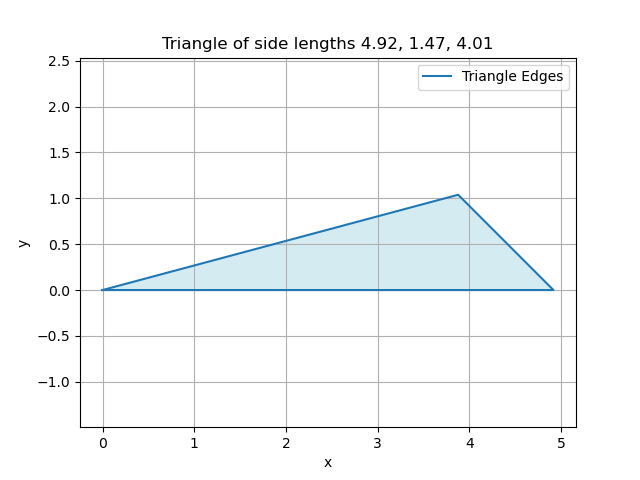
\includegraphics[width=0.8\linewidth]{figs/fig.png}
   	\caption{Triangle with $\angle B=45\degree$, $\angle C=120\degree$ and Perimeter = $10.4cm$}
\label{Plot}
\end{figure}
\end{document}
\end{document}
